\documentclass[10pt,a4paper]{article}
\usepackage[utf8]{inputenc}
\usepackage{amsmath}
\usepackage{amsfonts}
\usepackage{amssymb}
\usepackage{graphicx}
\usepackage{caption}
\usepackage{subcaption}
\usepackage{float}
\usepackage{minted}
\usepackage[top=1.0in, bottom=1.0in, left=0.75in, right=0.75in]{geometry}
\author{Chittaranjan Srinivas Swaminathan and Anders Wikstrom}
\title{Scortec ER-I Manipulator Control using Arduino Due}
\begin{document}
\maketitle
\tableofcontents
\section{Introduction}

\section{Description of task}
The Scortec ER-I is a 5-DOF manipulator from Eshed Robotec. The
control box is missing and a new controller is needed. For this
purpose, the Arduino Due board and a motor shield is used. \\

Figure \ref{fig:axes} shows a description of the axes on the manipulator.

\begin{figure}[H]
    \centering
    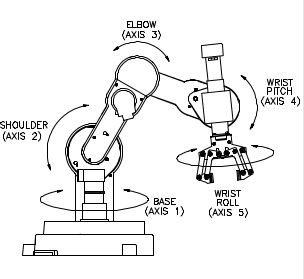
\includegraphics{axes.png}
    \caption{Description of axes}
    \label{fig:axes}
\end{figure}

The task of creating a controller for the manipulator involves the
following steps:
\begin{enumerate}
\item Reverse engineer the motor and encoder connections and make a
  pinout diagram for the D50 connector on the manipulator.
\item Program the microcontroller to read the encoders.
\item Write control routines for position and velocity control.
\item Extend the control routines to more than one joint.
\end{enumerate}

The following sections describe each of these tasks and challenges
faced while executing them.

\section{Reverse Engineering}

\subsection{Pinout}
\subsection{Encoders}
\subsection{Debouncing}

\section{Control routines}

\subsection{Calibration}
\subsection{Velocity Control}
\subsection{Position Control}
\subsection{Overall organization of code}

\section{Evaluation of the system}

\subsection{Calibration}
\subsection{Accuracy and Precision for Joint 1}

\section{Future Work}

\end{document}